\section{Results}

% TODO: Formatting.
\subsection{Delta Method}
Accuracy from 0 opponents to 10 opponents on PAN2013 dataset 1.

0.44943
0.58685
0.62235
0.63348
0.63741
0.63483
0.63876
0.64337
0.64123
0.64438
0.64235

Accuracy from 0 opponents to 10 opponents on PAN2013 dataset 2.

0.49606
0.58283
0.60125
0.60771
0.62173
0.61897
0.62787
0.63188
0.63488
0.63173
0.63291

Accuracy from 0 opponents to 10 opponents on PAN2015 dataset.

0.50000
0.55870
0.56550
0.53969
0.52880
0.52269
0.52080
0.51399
0.51270
0.51320
0.50840

\begin{figure}
    \centering
    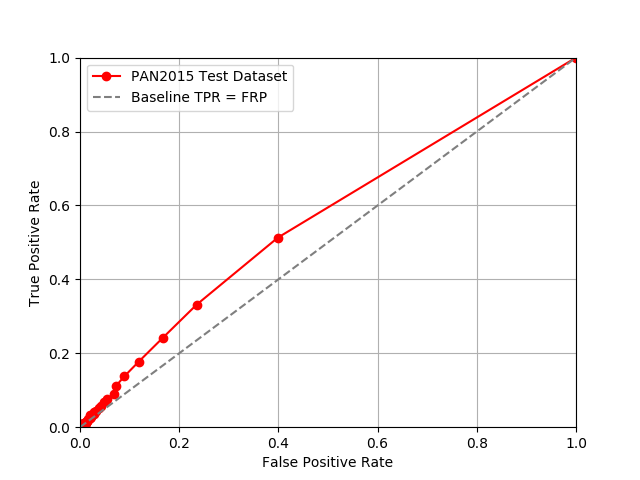
\includegraphics[width=.7\textwidth]{./pictures/delta_method_roc.png}
    \caption{The ROC curve of the delta method with number of opposing authors
    varying from 0 to 10 using the two test datasets for PAN2013 and the test
    dataset for PAN2015.}
    \label{fig:delta_method_roc}
\end{figure}

\subsection{Generalizing Random Forest}

\subsection{Extended Delta}

\subsection{Author Specific SVM}
% SVM performs well on binary authorship problems Abbasi & Chen, 2008; Zheng et al., 2006
% from https://pdfs.semanticscholar.org/5c2b/6876df693e096c6c150a5b0d2a2c05043003.pdf
